\documentclass[11pt, a4paper]{article}

% --- Packages ---
\usepackage[utf8]{inputenc} % Encoding
\usepackage{amsmath, amssymb, amsthm} % Advanced math typesetting
\usepackage{physics} % Useful commands for physics (derivatives, vectors, braket)
\usepackage{graphicx} % For including diagrams and images
\usepackage{geometry} % Page margins
\usepackage{siunitx} % For proper formatting of SI units
\usepackage{fancyhdr} % Custom headers and footers
\usepackage{xcolor} % For blocks of color
\usepackage{enumitem} % For enumerated lists with letters
\usepackage{float} % For figure strict positioning
\usepackage{parskip} % Elimina la sangría y añade espacio entre párrafos
\usepackage{booktabs} % For better table formatting
\usepackage{multirow} % For merging rows in tables
\usepackage{longtable} % For tables that span multiple pages
\usepackage{tikz} % For drawing diagrams
\usepackage{pgfplots} % For creating plots

% --- Page Setup ---
% --- Page Setup ---
\geometry{top=2.5cm, bottom=2.5cm, left=2.5cm, right=2.5cm}
\pagestyle{fancy}
\fancyhf{} % Clear all default header and footer fields
\fancyhead[L]{\textbf{José Carlos López Henestrosa}}
\fancyhead[R]{Inteligencia artificial - PEC3}
\fancyfoot[C]{\thepage} % Page number at the bottom center
\pgfplotsset{compat=1.17}

% --- Custom Environments ---
\newenvironment{problem}[1][Cuestión]{
	\vspace{0.5cm}
	\noindent{\Large\bfseries #1} \par\vspace{0.5cm}
}{
	\vspace{0.5cm}
}

\begin{document}
	% --- Title block ---
	\begin{center}
		\Large{ \textbf{PEC3} } \\
		\vspace{0.5cm}
		\normalsize{\textbf{Nombre:} José Carlos López Henestrosa} \\
		\vspace{0.5cm}
		\normalsize{Declaro que ostento la autoría total y llena de todas las tareas que se llevan a cabo en el presente documento. Soy la única persona que ha elaborado cada ejercicio. No he compartido los enunciados con nadie y la única ayuda que he recibido ha sido a través del aula de la UOC y su profesorado y he citado de forma explícita los recursos externos que he usado en la preparación de la PEC.} \\
		\vspace{0.5cm}
		\normalsize{Todas las referencias académicas en esta entrega hacen referencia al libro \textit{Sistemas basasdos en el conocimiento} de los recursos de esta asignatura, salvo que se cite otra fuente explícitamente.}
	\end{center}

	\vspace{1cm}
	\hrule
	\vspace{1cm}

	% --- Descripción de la PEC ---
	\begin{problem}[Descripción de la PEC a realizar]
		Se pide analizar el comportamiento de un sistema difuso jerárquico que se muestra a continuación:

		\begin{figure}[H]
			\centering
			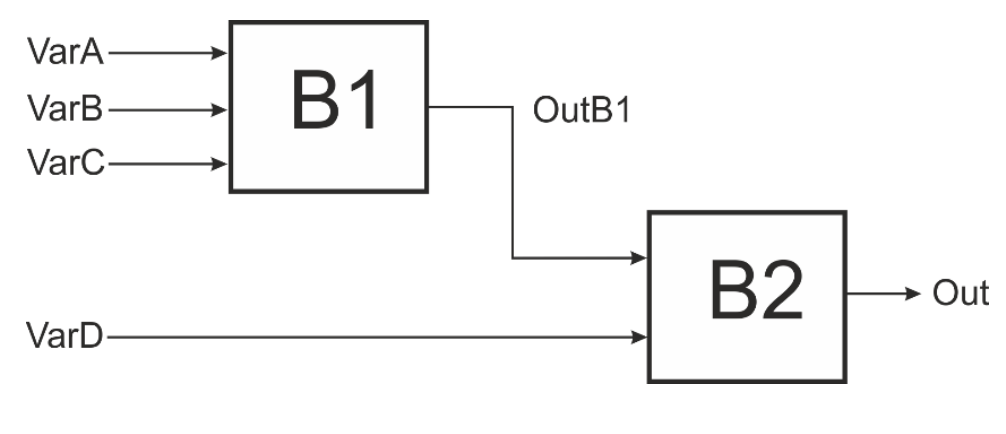
\includegraphics[width=13cm]{imagenes/descripcion_1.png}
			\caption{Sistema difuso}
		\end{figure}

		El sistema jerárquico está formado por 2 bloques de reglas (B1, B2) con 4 variables de entrada (VarA, VarB, VarC y VarD), 1 variable intermedia (OutB1) y 1 variable de salida (OutB2).

		Los dominios y los términos lingüísticos de las variables se presentan a continuación:

		\begin{table}[h]
			\centering
			\begin{tabular}{lll}
				\toprule
				\textbf{Variable} & \textbf{Rango} & \textbf{Término lingüístico: $(a,b,c,d)^{(*)}$} \\ \midrule
				\multirow{5}{*}{VarA} & Min: -5 & VL: (-5, -5, -5, 0) \\
				 & \multirow{4}{*}{Max: 5} & L: (-5, 0, 0, 2) \\
				 &  & M: (0, 2, 2, 4) \\
				 &  & H: (2, 4, 4, 5) \\
				 &  & VH: (4, 5, 5, 5) \\ \midrule
				\multirow{3}{*}{VarB} & Min: -5 & L: (-5, -5, -2, 2) \\
				 & \multirow{2}{*}{Max: 5} & M: (-1, 0, 0, 1) \\
				 &  & H: (-3, 2, 5, 5) \\ \midrule
				\multirow{3}{*}{VarC} & Min: 0 & L: (0, 0, 0, 8) \\
				 & \multirow{2}{*}{Max: 10} & M: (0, 8, 8, 10) \\
				 &  & H: (8, 10, 10, 10) \\ \midrule
				\multirow{5}{*}{VarD} & Min: 0 & VL: (0, 0, 0, 1) \\
				 & \multirow{4}{*}{Max: 10} & L: (0, 2, 2, 3) \\
				 &  & M: (2, 4, 5, 6) \\
				 &  & H: (5, 6, 6, 10) \\
				 &  & VH: (7, 8, 10, 10) \\ \midrule
				\multirow{5}{*}{OutB1, OutB2} & Min: -1 & VL: (-1, -1, -1, -0.8) \\
				 & \multirow{4}{*}{Max: 1} & L: (-1, -0.8, -0.8, -0.6) \\
				 &  & AM: (-0.8, -0.6, -0.6, 0.2) \\
				 &  & H: (-0.6, 0.2, 0.2, 1) \\
				 &  & VH: (0.2, 1, 1, 1) \\ \bottomrule
			\end{tabular}

			\vspace{0.5em}

			\small
			\begin{flushleft}
				$^{(*)}$ A continuación, la figura muestra la interpretación de la secuencia de puntos (a,b,c,d).

				Se presentan dos ejemplos ilustrativos, un término lingüístico trapezoidal (arriba) y un término lingüístico trigonal (debajo).
			\end{flushleft}
		\end{table}

		\begin{figure}[H]
			\centering
			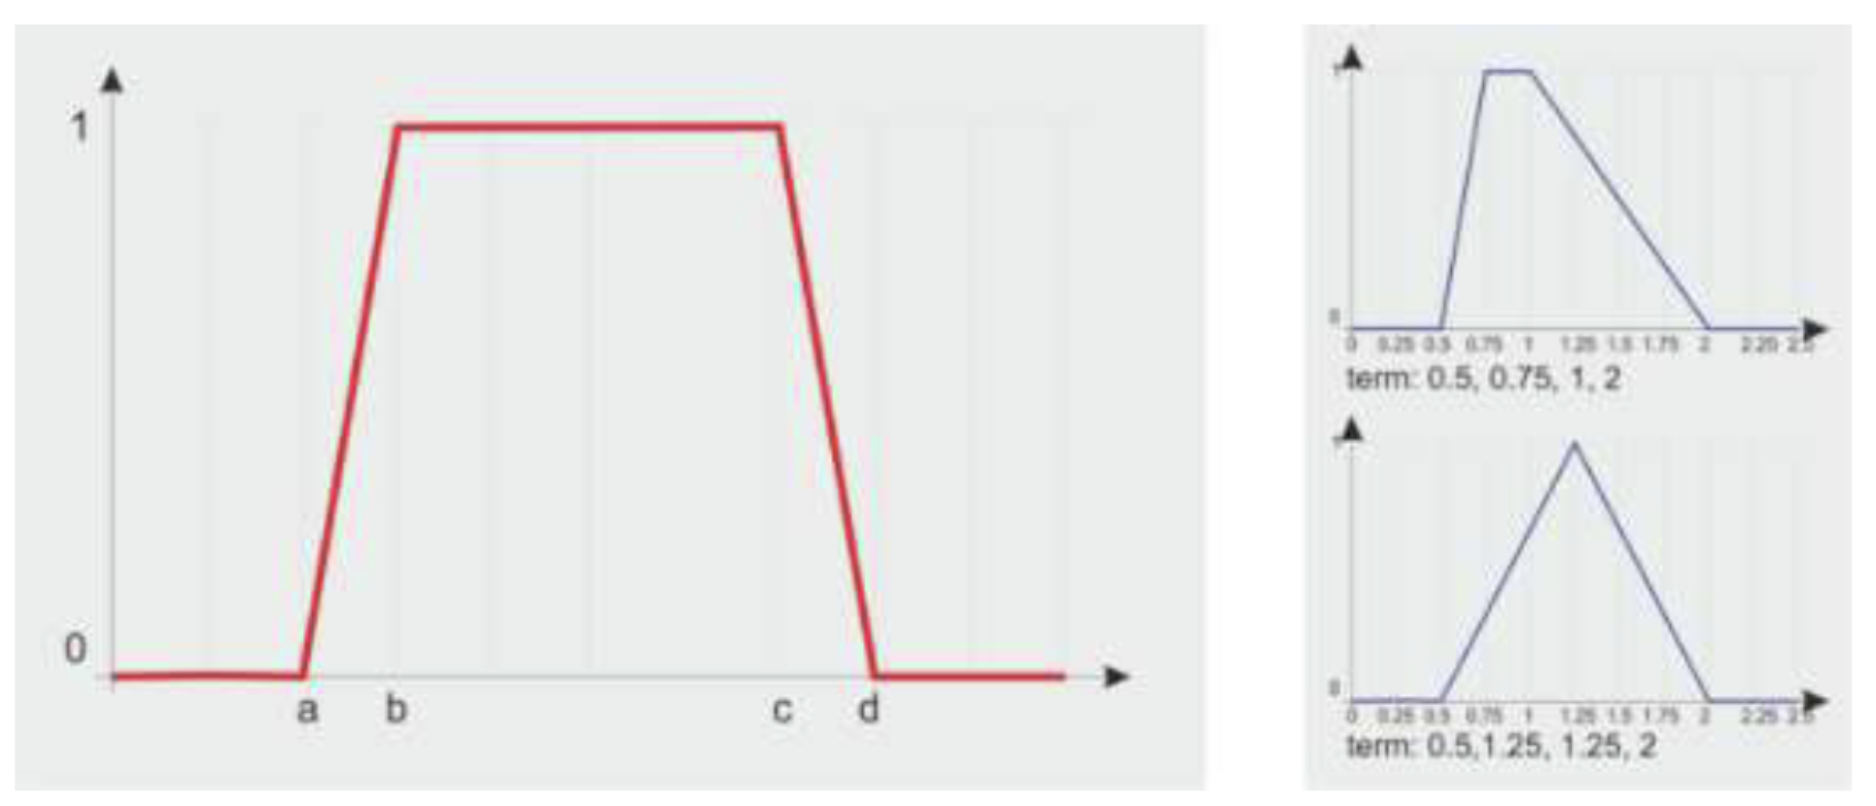
\includegraphics[width=13cm]{imagenes/descripcion_2.png}
			\caption{Términos lingüísticos}
		\end{figure}

		Las reglas del bloque B1 son las siguientes:

		\begin{longtable}{ccccccc}
			\toprule
			\textbf{Regla} & \textbf{VarA} & & \textbf{VarB} & & \textbf{VarC} & \textbf{OutB1} \\ \midrule
			\endfirsthead

			\multicolumn{7}{c}{{\bfseries \tablename\ \thetable{} -- continuación de la página anterior}} \\
			\toprule
			\textbf{Regla} & \textbf{VarA} & & \textbf{VarB} & & \textbf{VarC} & \textbf{OutB1} \\ \midrule
			\endhead

			\midrule
			\multicolumn{7}{r}{{Continúa en la siguiente página...}} \\
			\bottomrule
			\endfoot

			\bottomrule
			\endlastfoot

			01 & VL & AND & L & AND & L & VL \\
			02 & L & AND & L & AND & L & VL \\
			03 & M & AND & L & AND & L & L \\
			04 & H & AND & L & AND & L & L \\
			05 & VH & AND & L & AND & L & L \\
			06 & VL & AND & M & AND & L & L \\
			07 & L & AND & M & AND & L & AM \\
			08 & M & AND & M & AND & L & AM \\
			09 & H & AND & M & AND & L & AM \\
			10 & VH & AND & M & AND & L & AM \\
			11 & VL & AND & H & AND & L & AM \\
			12 & L & AND & H & AND & L & AM \\
			13 & M & AND & H & AND & L & H \\
			14 & H & AND & H & AND & L & H \\
			15 & VH & AND & H & AND & L & H \\
			16 & VL & AND & L & AND & M & L \\
			17 & L & AND & L & AND & M & L \\
			18 & M & AND & L & AND & M & L \\
			19 & H & AND & L & AND & M & AM \\
			20 & VH & AND & L & AND & M & H \\
			21 & VL & AND & M & AND & M & AM \\
			22 & L & AND & M & AND & M & AM \\
			23 & M & AND & M & AND & M & AM \\
			24 & H & AND & M & AND & M & AM \\
			25 & VH & AND & M & AND & M & AM \\
			26 & VL & AND & H & AND & M & AM \\
			27 & L & AND & H & AND & M & H \\
			28 & M & AND & H & AND & M & H \\
			29 & H & AND & H & AND & M & H \\
			30 & VH & AND & H & AND & M & H \\
			31 & VL & AND & L & AND & H & L \\
			32 & L & AND & L & AND & H & L \\
			33 & M & AND & L & AND & H & L \\
			34 & H & AND & L & AND & H & AM \\
			35 & VH & AND & L & AND & H & H \\
			36 & VL & AND & M & AND & H & AM \\
			37 & L & AND & M & AND & H & AM \\
			38 & M & AND & M & AND & H & AM \\
			39 & H & AND & M & AND & H & AM \\
			40 & VH & AND & M & AND & H & AM \\
			41 & VL & AND & H & AND & H & AM \\
			42 & L & AND & H & AND & H & AM \\
			43 & M & AND & H & AND & H & H \\
			44 & H & AND & H & AND & H & VH \\
			45 & VH & AND & H & AND & H & VH \\
		\end{longtable}

		Las reglas del bloque B2 son las siguientes:

		\begin{table}[h]
			\centering
			\caption{Base de reglas adicionales para OutB2}
			\begin{tabular}{ccccc}
				\toprule
				\textbf{Regla} & \textbf{OutB1} & & \textbf{VarD} & \textbf{OutB2} \\ \midrule
				01 & VL & AND & VL & VL \\
				02 &    &     & L  & VL \\
				03 & AM & AND & M  & L  \\
				04 & H  & AND & H  & AM \\
				05 & VH & AND & VH & VH \\
				06 &    &     & NOT(VL) & VH \\
				07 & L  & OR  & NOT(H)  & L  \\
				08 & VL & OR  & NOT(VH) & VL \\
				09 & VH & OR  & VH & VH \\
				10 & L  & AND & VL & L  \\
				11 & L  & AND & L  & L  \\
				12 & L  & AND & M  & L  \\ \bottomrule
			\end{tabular}
		\end{table}
	\end{problem}

	\textbf{Preguntas}

	Para el bloque B1 consideramos un sistema Madami con t-norma mínimo y t-conorma máximo:

	\begin{itemize}
		\item \textit{T}-norma: $T(a,b) = \min(a,b)$.
		\item \textit{T}-conorma: $S(a,b) = \max(a,b)$.
	\end{itemize}

	Para el bloque B2 consideramos un sistema con t-norma producto algebraico y t-conorma suma algebraica:

	\begin{itemize}
		\item \textit{T}-norma: $T(a,b) = ab$.
		\item \textit{T}-conorma: $S(a,b) = a + b - ab$.
	\end{itemize}

	El bloque de reglas B2 requiere una función de complementación. Considerar la siguiente función de la familia de Sugeno:

	$$N_{\lambda}(a)= (1-a) / (1 + \lambda a) \text{ considerando } \lambda = 2$$

	\begin{problem}[Problema 1 (20 \%)]
		Dar el detalle de las funciones de pertenencia de cada una de las variables del sistema (VarA, VarB, VarC, VarD y OutB1/OutB2)

		{ \color{blue} 
			Dado un término lingüístico definido por los puntos $a, b, c, d$, su función de pertenencia $\mu(x)$ trapezoidal (o triangular si $b=c$) se define de manera general como:

			\[
			\mu(x) = \begin{cases} 
			0 & \text{si } x \le a \\
			\frac{x-a}{b-a} & \text{si } a < x < b \\
			1 & \text{si } b \le x \le c \\
			\frac{d-x}{d-c} & \text{si } c < x < d \\
			0 & \text{si } x \ge d 
			\end{cases}
			\]

			Detallamos la definición analítica para cada una de las variables del sistema:

			\subsection*{Variable VarA (rango: $[-5, 5]$)}
				\begin{itemize}
					\item \textbf{VL} $(-5, -5, -5, 0)$:
						\[
						\mu_{VL}(x) = \begin{cases} 
						\frac{-x}{5} & \text{si } -5 \le x \le 0 \\ 
						0 & \text{en otro caso} 
						\end{cases}
						\]

					\item \textbf{L} $(-5, 0, 0, 2)$:
						\[
						\mu_{L}(x) = \begin{cases} 
						\frac{x+5}{5} & \text{si } -5 \le x \le 0 \\ 
						\frac{2-x}{2} & \text{si } 0 < x \le 2 \\ 
						0 & \text{en otro caso} 
						\end{cases}
						\]

					\item \textbf{M} $(0, 2, 2, 4)$:
						\[
						\mu_{M}(x) = \begin{cases} 
						\frac{x}{2} & \text{si } 0 \le x \le 2 \\ 
						\frac{4-x}{2} & \text{si } 2 < x \le 4 \\ 
						0 & \text{en otro caso} 
						\end{cases}
						\]

					\item \textbf{H} $(2, 4, 4, 5)$:
						\[
						\mu_{H}(x) = \begin{cases} 
						\frac{x-2}{2} & \text{si } 2 \le x \le 4 \\ 
						5-x & \text{si } 4 < x \le 5 \\ 
						0 & \text{en otro caso} 
						\end{cases}
						\]

					\item \textbf{VH} $(4, 5, 5, 5)$:
						\[
						\mu_{VH}(x) = \begin{cases} 
						x-4 & \text{si } 4 \le x \le 5 \\ 
						0 & \text{en otro caso} 
						\end{cases}
						\]
				\end{itemize}

			\subsection*{Variable VarB (rango: $[-5, 5]$)}
				\begin{itemize}
					\item \textbf{L} $(-5, -5, -2, 2)$:
						\[
						\mu_{L}(x) = \begin{cases} 
						1 & \text{si } -5 \le x \le -2 \\ 
						\frac{2-x}{4} & \text{si } -2 < x \le 2 \\ 
						0 & \text{en otro caso} 
						\end{cases}
						\]

					\item \textbf{M} $(-1, 0, 0, 1)$:
						\[
						\mu_{M}(x) = \begin{cases} 
						x+1 & \text{si } -1 \le x \le 0 \\ 
						1-x & \text{si } 0 < x \le 1 \\ 
						0 & \text{en otro caso} 
						\end{cases}
						\]

					\item \textbf{H} $(-3, 2, 5, 5)$:
						\[
						\mu_{H}(x) = \begin{cases} 
						\frac{x+3}{5} & \text{si } -3 \le x \le 2 \\ 
						1 & \text{si } 2 < x \le 5 \\ 
						0 & \text{en otro caso} 
						\end{cases}
						\]
				\end{itemize}

			\subsection*{Variable VarC (rango: $[0,10]$)}
				\begin{itemize}
					\item \textbf{L} $(0, 0, 0, 8)$:
						\[
						\mu_{L}(x) = \begin{cases} 
						\frac{8-x}{8} & \text{si } 0 \le x \le 8 \\ 
						0 & \text{en otro caso} 
						\end{cases}
						\]

					\item \textbf{M} $(0, 8, 8, 10)$:
						\[
						\mu_{M}(x) = \begin{cases} 
						\frac{x}{8} & \text{si } 0 \le x \le 8 \\ 
						\frac{10-x}{2} & \text{si } 8 < x \le 10 \\ 
						0 & \text{en otro caso} 
						\end{cases}
						\]

					\item \textbf{H} $(8, 10, 10, 10)$:
						\[
						\mu_{H}(x) = \begin{cases} 
						\frac{x-8}{2} & \text{si } 8 \le x \le 10 \\ 
						0 & \text{en otro caso} 
						\end{cases}
						\]
				\end{itemize}

			\subsection*{Variable VarD (rango: $[0,10]$)}
				\begin{itemize}
					\item \textbf{VL} $(0, 0, 0, 1)$:
						\[
						\mu_{VL}(x) = \begin{cases} 
						1-x & \text{si } 0 \le x \le 1 \\ 
						0 & \text{en otro caso} 
						\end{cases}
						\]

					\item \textbf{L} $(0, 2, 2, 3)$:
						\[
						\mu_{L}(x) = \begin{cases} 
						\frac{x}{2} & \text{si } 0 \le x \le 2 \\ 
						3-x & \text{si } 2 < x \le 3 \\ 
						0 & \text{en otro caso} 
						\end{cases}
						\]

					\item \textbf{M} $(2, 4, 5, 6)$:
						\[
						\mu_{M}(x) = \begin{cases} 
						\frac{x-2}{2} & \text{si } 2 \le x \le 4 \\ 
						1 & \text{si } 4 < x \le 5 \\ 
						6-x & \text{si } 5 < x \le 6 \\ 
						0 & \text{en otro caso} 
						\end{cases}
						\]

					\item \textbf{H} $(5, 6, 6, 10)$:
						\[
						\mu_{H}(x) = \begin{cases} 
						x-5 & \text{si } 5 \le x \le 6 \\ 
						\frac{10-x}{4} & \text{si } 6 < x \le 10 \\ 
						0 & \text{en otro caso} 
						\end{cases}
						\]

					\item \textbf{VH} $(7, 8, 10, 10)$:
						\[
						\mu_{VH}(x) = \begin{cases} 
						x-7 & \text{si } 7 \le x \le 8 \\ 
						1 & \text{si } 8 < x \le 10 \\ 
						0 & \text{en otro caso} 
						\end{cases}
						\]
				\end{itemize}

			\subsection*{Variables OutB1, OutB2 (rango: $[-1, 1]$)}
				\begin{itemize}
					\item \textbf{VL} $(-1, -1, -1, -0.8)$:
						\[
						\mu_{VL}(x) = \begin{cases} 
						\frac{-0.8-x}{0.2} & \text{si } -1 \le x \le -0.8 \\ 
						0 & \text{en otro caso} 
						\end{cases}
						\]

					\item \textbf{L} $(-1, -0.8, -0.8, -0.6)$:
						\[
						\mu_{L}(x) = \begin{cases} 
						\frac{x+1}{0.2} & \text{si } -1 \le x \le -0.8 \\ 
						\frac{-0.6-x}{0.2} & \text{si } -0.8 < x \le -0.6 \\ 
						0 & \text{en otro caso} 
						\end{cases}
						\]

					\item \textbf{AM} $(-0.8, -0.6, -0.6, 0.2)$:
						\[
						\mu_{AM}(x) = \begin{cases} 
						\frac{x+0.8}{0.2} & \text{si } -0.8 \le x \le -0.6 \\ 
						\frac{0.2-x}{0.8} & \text{si } -0.6 < x \le 0.2 \\ 
						0 & \text{en otro caso} 
						\end{cases}
						\]

					\item \textbf{H} $(-0.6, 0.2, 0.2, 1)$:
						\[
						\mu_{H}(x) = \begin{cases} 
						\frac{x+0.6}{0.8} & \text{si } -0.6 \le x \le 0.2 \\ 
						\frac{1-x}{0.8} & \text{si } 0.2 < x \le 1 \\ 
						0 & \text{en otro caso} 
						\end{cases}
						\]

					\item \textbf{VH} $(0.2, 1, 1, 1)$:
						\[
						\mu_{VH}(x) = \begin{cases} 
						\frac{x-0.2}{0.8} & \text{si } 0.2 \le x \le 1 \\ 
						0 & \text{en otro caso} 
						\end{cases}
						\]
				\end{itemize}
		}
	\end{problem}

	% --- Exercise 2 ---
	\begin{problem}[Problema 2 (60 \%)]
		Se pide dar la salida gráfica del proceso de inferencia, indicando las reglas activadas, para los siguientes valores de entrada:

		$$\text{(VarA, VarB, VarC, VarD)} = (-1,0.5,5.5,7.5)$$

		{ \color{blue} 
			En primer lugar, realizamos el proceso de \textbf{fuzzificación}, en el que evaluamos el grado de pertenencia $\mu$ de cada valor nítido en sus respectivos términos lingüísticos. Para obtenerlos, evaluamos cada valor nítido de entrada en las funciones de pertenencia definidas previamente. La pertenencia será mayor que $0$ solo si el valor de entrada $x$ se encuentra dentro del intervalo de definición $(a, d)$ del término lingüístico correspondiente.

			Desglosamos el cálculo por variable:

			\subsubsection*{Variable VarA ($x = -1$)}
				El valor $x = -1$ se encuentra en el rango $[-5, 0]$. Revisamos qué términos están definidos en dicho intervalo:

				\begin{itemize}
					\item \textbf{Término VL} $(-5, -5, -5, 0)$: En el tramo de bajada $(-5 \le x \le 0)$, la función es $\frac{-x}{5}$.
						\[ \mu_{VL}(-1) = \frac{-(-1)}{5} = \frac{1}{5} = \mathbf{0.2} \]

					\item \textbf{Término L} $(-5, 0, 0, 2)$: En el tramo de subida $(-5 \le x \le 0)$, la función es $\frac{x+5}{5}$.
						\[ \mu_{L}(-1) = \frac{-1+5}{5} = \frac{4}{5} = \mathbf{0.8} \]
				\end{itemize}

				Para los términos M, H y VH, el valor $-1$ está fuera de sus dominios, por lo que su grado de pertenencia es $0$.

			\subsubsection*{Variable VarB ($x = 0.5$)}
				El valor $x = 0.5$ incide en los tres conjuntos definidos para VarB, por lo que evaluamos la función correspondiente en el tramo adecuado para cada uno:

				\begin{itemize}
					\item \textbf{Término L} $(-5, -5, -2, 2)$: En el tramo de bajada $(-2 < x \le 2)$, la ecuación es $\frac{2-x}{4}$.
						\[ \mu_{L}(0.5) = \frac{2 - 0.5}{4} = \frac{1.5}{4} = \mathbf{0.375} \]

					\item \textbf{Término M} $(-1, 0, 0, 1)$: En el tramo de bajada $(0 < x \le 1)$, la ecuación es $1-x$.
						\[ \mu_{M}(0.5) = 1 - 0.5 = \mathbf{0.5} \]

					\item \textbf{Término H} $(-3, 2, 5, 5)$: En el tramo de subida $(-3 \le x \le 2)$, la ecuación es $\frac{x+3}{5}$.
						\[ \mu_{H}(0.5) = \frac{0.5+3}{5} = \frac{3.5}{5} = \mathbf{0.7} \]
				\end{itemize}

			\subsubsection*{Variable VarC ($x = 5.5$)}
				El valor $x = 5.5$ está dentro del intervalo $[2]$. En este tramo tienen presencia los términos L y M:

				\begin{itemize}
					\item \textbf{Término L} $(0, 0, 0, 8)$: En su tramo de bajada $(0 \le x \le 8)$, la función es $\frac{8-x}{8}$.
						\[ \mu_{L}(5.5) = \frac{8 - 5.5}{8} = \frac{2.5}{8} = \mathbf{0.3125} \]

					\item \textbf{Término M} $(0, 8, 8, 10)$: En el tramo de subida $(0 \le x \le 8)$, la función es $\frac{x}{8}$.
						\[ \mu_{M}(5.5) = \frac{5.5}{8} = \mathbf{0.6875} \]
				\end{itemize}

				El término H empieza en $x=8$, por lo que su pertenencia para $5.5$ es $0$.

			\subsubsection*{Variable VarD ($x = 7.5$)}
				El valor $x = 7.5$ es mayor que $6$, afectando a la parte alta del dominio donde residen los términos H y VH:

				\begin{itemize}
					\item \textbf{Término H} $(5, 6, 6, 10)$: En su tramo de bajada $(6 < x \le 10)$, la función es $\frac{10-x}{4}$.
						\[ \mu_{H}(7.5) = \frac{10 - 7.5}{4} = \frac{2.5}{4} = \mathbf{0.625} \]

					\item \textbf{Término VH} $(7, 8, 10, 10)$: En el tramo de subida $(7 \le x \le 8)$, la función es $x-7$.
						\[ \mu_{VH}(7.5) = 7.5 - 7 = \mathbf{0.5} \]
				\end{itemize}

				Para el resto de los términos (VL, L, M) sus dominios terminan antes o en el $6$, por lo que para $x=7.5$ la pertenencia es exactamente $0$.

				Una vez obtenidos estos grados, continuamos con la \textbf{inferencia del Bloque 1 (B1)} utilizando el método de Mamdani con la t-norma del mínimo (AND) para evaluar los antecedentes y la t-conorma del máximo (OR) para la agregación de las conclusiones. Las reglas activadas, las cuales son aquellas con grado $> 0$ y sus conclusiones truncadas son las siguientes:

				\begin{table}[H]
					\centering
					\color{blue}
					\begin{tabular}{clc}
						\toprule
						\textbf{Regla} & \textbf{Antecedentes (VarA AND VarB AND VarC)} & \textbf{Activación (mínimo) $\rightarrow$ OutB1} \\
						\midrule
						R01 & VL(0.2) AND L(0.375) AND L(0.3125) & $0.2 \rightarrow$ \textbf{VL} \\
						R02 & L(0.8) AND L(0.375) AND L(0.3125) & $0.3125 \rightarrow$ \textbf{VL} \\
						R06 & VL(0.2) AND M(0.5) AND L(0.3125) & $0.2 \rightarrow$ \textbf{L} \\
						R07 & L(0.8) AND M(0.5) AND L(0.3125) & $0.3125 \rightarrow$ \textbf{AM} \\
						R11 & VL(0.2) AND H(0.7) AND L(0.3125) & $0.2 \rightarrow$ \textbf{AM} \\
						R12 & L(0.8) AND H(0.7) AND L(0.3125) & $0.3125 \rightarrow$ \textbf{AM} \\
						R16 & VL(0.2) AND L(0.375) AND M(0.6875) & $0.2 \rightarrow$ \textbf{L} \\
						R17 & L(0.8) AND L(0.375) AND M(0.6875) & $0.375 \rightarrow$ \textbf{L} \\
						R21 & VL(0.2) AND M(0.5) AND M(0.6875) & $0.2 \rightarrow$ \textbf{AM} \\
						R22 & L(0.8) AND M(0.5) AND M(0.6875) & $0.5 \rightarrow$ \textbf{AM} \\
						R26 & VL(0.2) AND H(0.7) AND M(0.6875) & $0.2 \rightarrow$ \textbf{AM} \\
						R27 & L(0.8) AND H(0.7) AND M(0.6875) & $0.6875 \rightarrow$ \textbf{H} \\
						\bottomrule
					\end{tabular}
				\end{table}

				Tras la agregación mediante la t-conorma del máximo, obtenemos los grados de activación para los conjuntos difusos de la variable \textbf{OutB1}, los cuales son los siguientes:

				\begin{itemize}
					\item \textbf{VL}: $\max(0.2, 0.3125) = 0.3125$
					\item \textbf{L}: $\max(0.2, 0.2, 0.375) = 0.375$
					\item \textbf{AM}: $\max(0.3125, 0.2, 0.3125, 0.2, 0.5, 0.2) = 0.5$
					\item \textbf{H}: $\max(0.6875) = 0.6875$
					\item \textbf{VH}: $0$
				\end{itemize}

				Posteriormente, el \textbf{Bloque 2 (B2)} aplica una lógica distinta basada en el producto algebraico para la t-norma y la suma algebraica para la t-conorma, junto al complemento de Sugeno $\left ( N(x) = \frac{1-x}{1+2x} \right )$, tal que así:

				\begin{itemize}
					\item \textbf{T-norma (AND)}: Producto algebraico $T(a,b) = a \cdot b$.
					\item \textbf{T-conorma (OR)}: Suma algebraica $S(a,b) = a + b - a \cdot b$.
					\item \textbf{Complemento (NOT)}: Familia de Sugeno con $\lambda = 2 \implies N(x) = \frac{1-x}{1+2x}$.
				\end{itemize}

				Aplicamos estas operaciones a las reglas de B2 evaluando los antecedentes de las reglas activadas (OutB1 y VarD):

				\begin{table}[H]
					\centering
					\color{blue}
					\begin{tabular}{clc}
						\toprule
						\textbf{Regla} & \textbf{Evaluación del antecedente} & \textbf{Conclusión $\rightarrow$ OutB2} \\
						\midrule
						R04 & \textbf{OutB1\_H AND VarD\_H} \\
							& $0.6875 \cdot 0.625 = 0.4296875$ & $\rightarrow$ \textbf{AM (0.4296875)} \\
						\midrule
						R06 & \textbf{NOT(VarD\_VL)} \\
							& $N(0) = \frac{1-0}{1+0} = 1.0$ & $\rightarrow$ \textbf{VH (1.0)} \\
						\midrule
						R07 & \textbf{OutB1\_L OR NOT(VarD\_H)} \\
							& $N(0.625) = \frac{1-0.625}{1+1.25} = 0.166667$ \\
							& $S(0.375, 0.166667) = 0.375 + 0.166667 - (0.375 \cdot 0.166667) = 0.479167$ & $\rightarrow$ \textbf{L (0.479167)} \\
						\midrule
						R08 & \textbf{OutB1\_VL OR NOT(VarD\_VH)} \\
							& $N(0.5) = \frac{1-0.5}{1+1} = 0.25$ \\
							& $S(0.3125, 0.25) = 0.3125 + 0.25 - (0.3125 \cdot 0.25) = 0.484375$ & $\rightarrow$ \textbf{VL (0.484375)} \\
						\midrule
						R09 & \textbf{OutB1\_VH OR VarD\_VH} \\
							& $S(0, 0.5) = 0 + 0.5 - 0 = 0.5$ & $\rightarrow$ \textbf{VH (0.5)} \\
						\bottomrule
					\end{tabular}
				\end{table}

				Dado que para el término \textbf{VH} se han activado dos reglas distintas, R06 y R09, sumamos sus valores utilizando la t-conorma de la suma algebraica:

				\[
				\alpha_{VH} = S(1.0, 0.5) = 1.0 + 0.5 - (1.0 \cdot 0.5) = 1.0
				\]

				En este sistema, mediante la inferencia del producto, la activación $\alpha$ de la regla escala el conjunto difuso del consecuente en lugar de truncarlo, como ocurre con el mínimo. 

				Los grados finales de escalado para OutB2 son: 

				\begin{itemize}
					\item \textbf{VL} = 0.484
					\item \textbf{L} = 0.479
					\item \textbf{AM} = 0.430
					\item \textbf{H} = 0
					\item \textbf{VH} = 1.0
				\end{itemize}

				\newpage

				Por último, \textbf{presentamos las gráficas} resultantes de este proceso. La primera enseña la variable intermedia \textbf{OutB1} truncada por la t-norma del mínimo, y la segunda gráfica ilustra la salida final \textbf{OutB2} escalada mediante el producto algebraico.

				\vspace{0.5cm}

				\begin{center}
					\textbf{Variable OutB1 truncada} \\
					\vspace{0.3cm}
					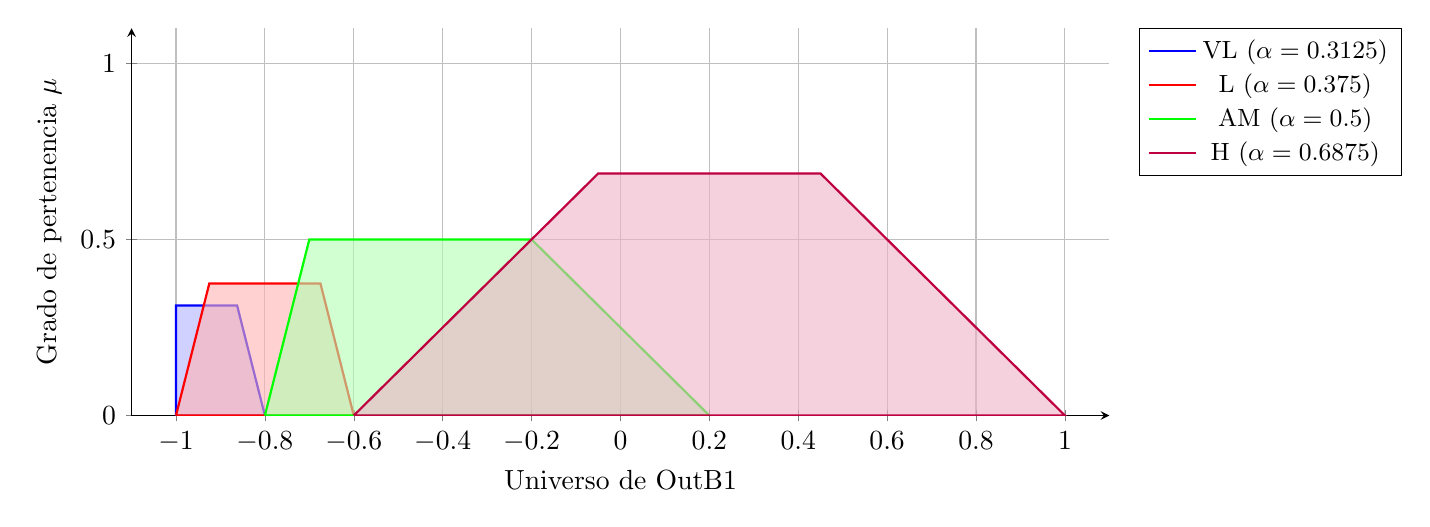
\begin{tikzpicture}
						\begin{axis}[
							width=14cm, height=6.5cm,
							xmin=-1.1, xmax=1.1,
							ymin=0, ymax=1.1,
							axis lines=left,
							xlabel={Universo de OutB1},
							ylabel={Grado de pertenencia $\mu$},
							grid=major,
							legend pos=outer north east,
							legend style={font=\small}
						]
							% OutB1_VL
							\addplot[fill=blue!30, draw=blue, thick, fill opacity=0.6] coordinates {(-1, 0) (-1, 0.3125) (-0.8625, 0.3125) (-0.8, 0) (-1, 0)};
							\addlegendentry{VL ($\alpha=0.3125$)}
							% OutB1_L
							\addplot[fill=red!30, draw=red, thick, fill opacity=0.6] coordinates {(-1, 0) (-0.925, 0.375) (-0.675, 0.375) (-0.6, 0) (-1, 0)};
							\addlegendentry{L ($\alpha=0.375$)}
							% OutB1_AM
							\addplot[fill=green!30, draw=green, thick, fill opacity=0.6] coordinates {(-0.8, 0) (-0.7, 0.5) (-0.2, 0.5) (0.2, 0) (-0.8, 0)};
							\addlegendentry{AM ($\alpha=0.5$)}
							% OutB1_H
							\addplot[fill=purple!30, draw=purple, thick, fill opacity=0.6] coordinates {(-0.6, 0) (-0.05, 0.6875) (0.45, 0.6875) (1, 0) (-0.6, 0)};
							\addlegendentry{H ($\alpha=0.6875$)}
						\end{axis}
					\end{tikzpicture}

					\vspace{1cm}

					\textbf{Variable OutB2 escalada} \\

					\vspace{0.3cm}

					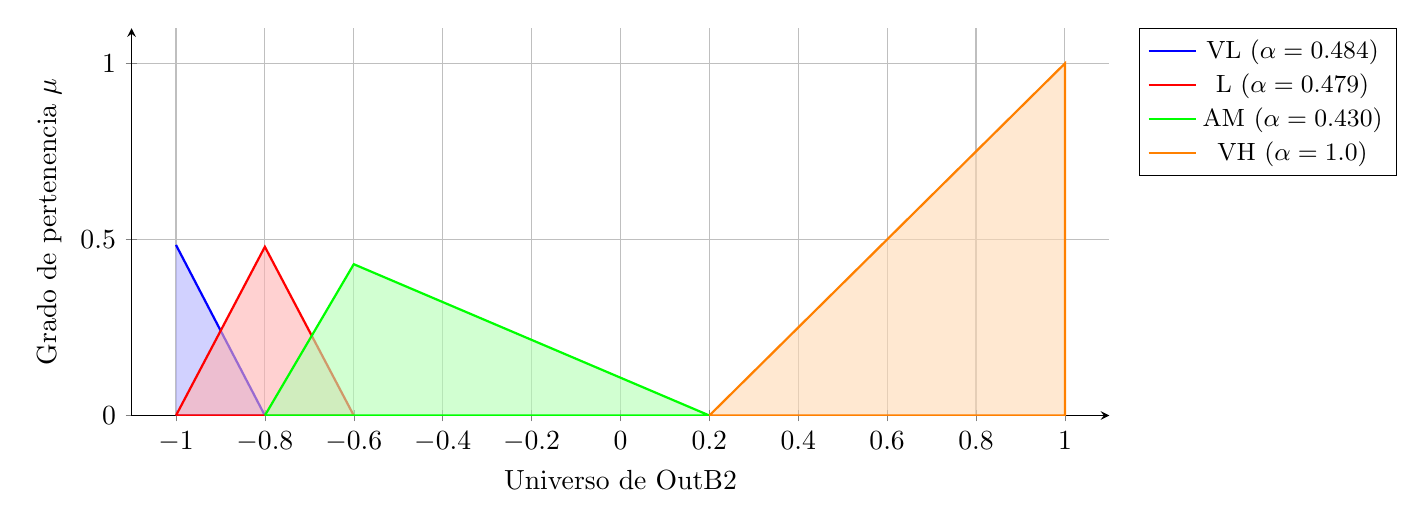
\begin{tikzpicture}
						\begin{axis}[
							width=14cm, height=6.5cm,
							xmin=-1.1, xmax=1.1,
							ymin=0, ymax=1.1,
							axis lines=left,
							xlabel={Universo de OutB2},
							ylabel={Grado de pertenencia $\mu$},
							grid=major,
							legend pos=outer north east,
							legend style={font=\small}
						]
							% OutB2_VL
							\addplot[fill=blue!30, draw=blue, thick, fill opacity=0.6] coordinates {(-1, 0.4844) (-0.8, 0) (-1, 0)};
							\addlegendentry{VL ($\alpha=0.484$)}
							% OutB2_L
							\addplot[fill=red!30, draw=red, thick, fill opacity=0.6] coordinates {(-1, 0) (-0.8, 0.4792) (-0.6, 0) (-1, 0)};
							\addlegendentry{L ($\alpha=0.479$)}
							% OutB2_AM
							\addplot[fill=green!30, draw=green, thick, fill opacity=0.6] coordinates {(-0.8, 0) (-0.6, 0.4297) (0.2, 0) (-0.8, 0)};
							\addlegendentry{AM ($\alpha=0.430$)}
							% OutB2_VH
							\addplot[fill=orange!30, draw=orange, thick, fill opacity=0.6] coordinates {(0.2, 0) (1, 1) (1, 0) (0.2, 0)};
							\addlegendentry{VH ($\alpha=1.0$)}
						\end{axis}
					\end{tikzpicture}
				\end{center}
		}
	\end{problem}

	% --- Exercise 3 ---

	\begin{problem}[Cuestión 3 (20 \%)]
		Se pide dar la salida nítida del sistema para las entradas de la pregunta anterior.

		Podéis usar cualquiera de los dos métodos, aproximado o analítico.

		{ \color{blue} 
			Para obtener el valor concreto de la variable de salida final \textbf{OutB2}, los sistemas difusos añaden un paso de \textbf{nitidificación} que consiste en obtener un valor nítido a partir de un conjunto difuso. Una de las formas de realizarlo es mediante el centro de masas (o centro de área) aproximado, que calcula una media de los valores discretizados del dominio ponderada por su grado de pertenencia al conjunto.

			La expresión matemática que rige este cálculo es:

			\[
			z^* = \frac{\sum_{i} x_i \cdot \mu_{OutB2}(x_i)}{\sum_{i} \mu_{OutB2}(x_i)}
			\]

			Comenzamos, pues, el procedimiento recuperando los grados de activación de la variable de salida obtenidos en la inferencia anterior:

			\begin{itemize}
				\item $\alpha_{VL} = 0.484$
				\item $\alpha_{L} = 0.479$
				\item $\alpha_{AM} = 0.430$
				\item $\alpha_{H} = 0$
				\item $\alpha_{VH} = 1.0$
			\end{itemize}

			A continuación, \textbf{discretizamos el universo de discurso de la variable \textbf{OutB2}}, definido en el intervalo $[-1, 1]$, utilizando pasos regulares de $\Delta x = 0.2$. Para cada punto $x_i$, evaluamos su pertenencia al conjunto final $\mu_{OutB2}(x_i)$ basándonos en la superposición de los conjuntos difusos individuales. Al haber truncado/escalado, la pertenencia en un punto concreto es directamente el valor original en ese punto multiplicado por el nivel de activación correspondiente de la regla:

			\begin{table}[H]
				\centering
				\color{blue}
				\begin{tabular}{c c c c}
					\toprule
					\textbf{$x_i$} & \textbf{Conjunto activo y evaluación} & \textbf{$\mu_{OutB2}(x_i)$} & \textbf{$x_i \cdot \mu_{OutB2}(x_i)$} \\
					\midrule
					-1.0 & VL (1.00) $\rightarrow 1.00 \cdot 0.484$ & 0.4840 & -0.4840 \\
					-0.8 & L (1.00) $\rightarrow 1.00 \cdot 0.479$ & 0.4790 & -0.3832 \\
					-0.6 & AM (1.00) $\rightarrow 1.00 \cdot 0.430$ & 0.4300 & -0.2580 \\
					-0.4 & AM (0.75) $\rightarrow 0.75 \cdot 0.430$ & 0.3225 & -0.1290 \\
					-0.2 & AM (0.50) $\rightarrow 0.50 \cdot 0.430$ & 0.2150 & -0.0430 \\
					 0.0 & AM (0.25) $\rightarrow 0.25 \cdot 0.430$ & 0.1075 &  0.0000 \\
					 0.2 & - & 0.0000 &  0.0000 \\
					 0.4 & VH (0.25) $\rightarrow 0.25 \cdot 1.00$ & 0.2500 &  0.1000 \\
					 0.6 & VH (0.50) $\rightarrow 0.50 \cdot 1.00$ & 0.5000 &  0.3000 \\
					 0.8 & VH (0.75) $\rightarrow 0.75 \cdot 1.00$ & 0.7500 &  0.6000 \\
					 1.0 & VH (1.00) $\rightarrow 1.00 \cdot 1.00$ & 1.0000 &  1.0000 \\
					\bottomrule
				\end{tabular}
			\end{table}

			\textit{Nota: En los puntos donde interactúa el término H, como su grado de activación ha resultado ser $\alpha_{H} = 0$, su contribución al cálculo es nula.}

			A continuación, realizamos las sumatorias necesarias para aplicar la fórmula de nitidificación del centro de masas. Dividimos el cálculo por el numerador y el denominador para que el proceso quede más claro:

			\paragraph{Numerador (suma de los momentos):}
			\[
			\sum_{i} x_i \cdot \mu_{OutB2}(x_i) = -0.484 - 0.3832 - 0.258 - 0.129 - 0.043 + 0 + 0 + 0.1 + 0.3 + 0.6 + 1.0 = \mathbf{0.7028}
			\]

			\paragraph{Denominador (suma del área difusa):}
			\[
			\sum_{i} \mu_{OutB2}(x_i) = 0.484 + 0.479 + 0.430 + 0.3225 + 0.215 + 0.1075 + 0 + 0.25 + 0.5 + 0.75 + 1.0 = \mathbf{4.538}
			\]

			\paragraph{Salida nítida final ($z^*$):}
			\[
			z^* = \frac{0.7028}{4.538} \approx \mathbf{0.1548}
			\]

			Como conclusión, sabemos que al aplicar el método aproximado de defuzzificación por centro de masas, la salida nítida de nuestro sistema para los valores de entrada iniciales $(-1, 0.5, 5.5, 7.5)$ es aproximadamente \textbf{0.1548}.
		}
	\end{problem}
\end{document}